\section{Overtoner}
Nu skal vi til at se lidt mere på hvad overtoner er og kan. Måske overvejer du, om overtoner overhovedet er en fysisk ting. Var det ikke bare et matematisk trick? Det korte svar er, at de "findes i virkeligheden", og det kommer vi til at se nogle eksempler på, både som matematik og vi vil også spille noget lyd for jer på emnet, hvor man kommer til at kunne høre nogle af de seje fænomener, som bl.a. kommer af overtoner. På figur \ref{aku:fig:D3} ses et eksempel på en trykbølge og dens tilsvarende overtonespektrum. Højden på hver pind viser, hvor kraftig den enkelte overtone er i forhold til de andre. Spektret er beregnet som en form for Fourier-spektrum, hvor hver enkelt overtone er et led i fourier-rækken. Højden af pinden er således matematisk set størrelsen af koefficienten på det tilsvarende led i fourier-summen, altså $C_n$ i \eqref{aku:eq:losning_2}.
\begin{figure}[t]
    \centering
    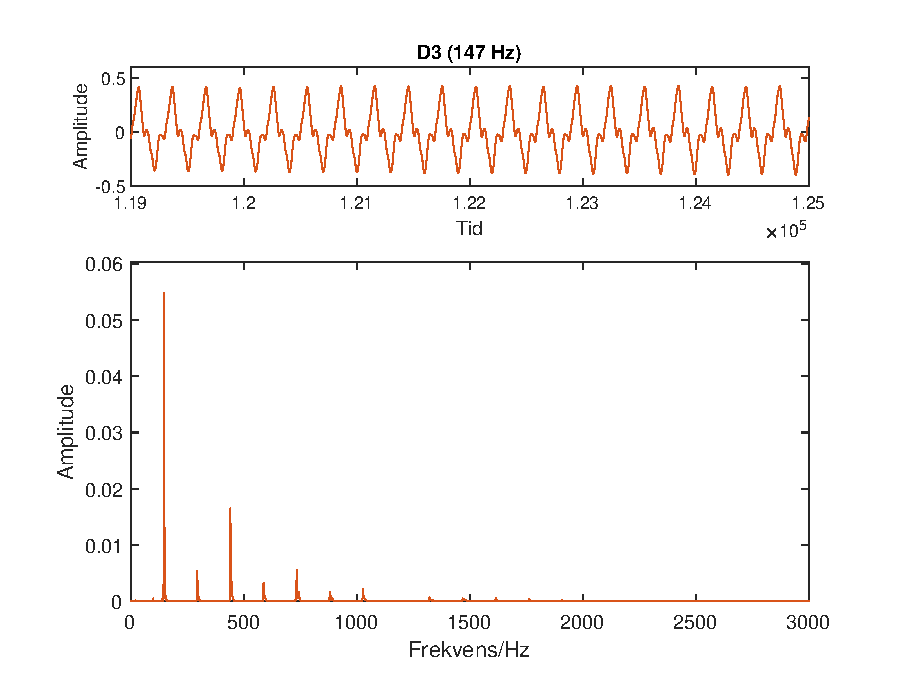
\includegraphics{Akustik/fig/D3.eps}
    \caption{Bølgeform og overtonespektrum af den dybeste tone på en klarinet, 147 \si{.Hz}}
    \label{aku:fig:D3}
\end{figure}
Bare ved at så på spektret kan man allerede få meget information - alle instrumenter (og fx stemmer) har forskellige forhold mellem hvor kraftige hver enkelt overtone er, og det er med til at give dem forskellig klang, altså gøre at de lyder forskelligt, selvom de spiller/synger samme tone. Selv det samme instrument kan lyde vidt forskelligt i forskellige registre, altså forskellige tonehøjdeområder.\footnote{Det højere register er alle toner der fremkommer ved en \textit{overblæsning} af tonerne i det lavere register, dvs. at alle tonerne i det højere register har grundtoner som er første overtone i det lavere register, eller set på en anden måde: tag det dybe register og fjern grundtonen: så får man det næste register. Dvs. et register er så mange toner som der er indtil man når første overtone for den dybeste tone i registeret.} Se bare den samme klarinet tre oktaver over på figur \ref{aku:fig:D6}.
\begin{figure}[t]
    \centering
    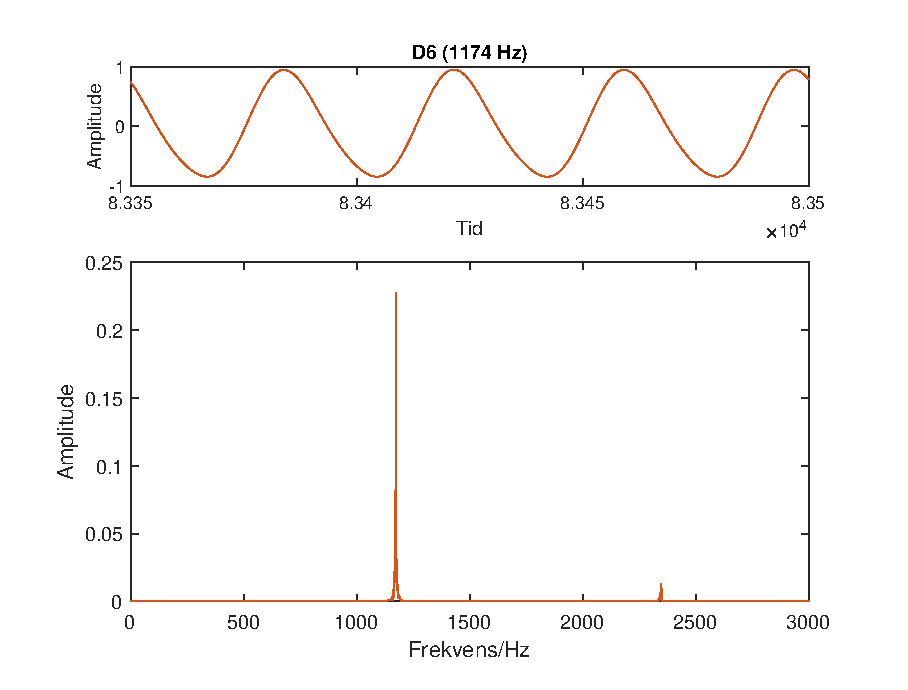
\includegraphics{Akustik/fig/D6.eps}
    \caption{Bølgeform og overtonespektrum på klarinet for en høj tone, 1174 \si{.Hz}.}
    \label{aku:fig:D6}
\end{figure}
Lad os nu betragte figur \ref{aku:fig:D3}. Ser det ud som om, der er et mønster i hvilke overtoner, der er kraftige, og hvilke der er mindre kraftige? Ja, hver anden overtone er der næsten ikke. Hvorfor det? For at finde svaret, er vi nødt til at kigge tilbage på, hvilke kriterier, der blev brugt for at løse bølgeligningen. Det viser sig nemlig, at der for en klarinet og en streng har forskellige randbetingelser. Hvor vi for strengen havde at hastigheden er 0 i begge ender af strengen får vi noget andet for blæsere. Hvor det for strengen gav mest mening at regne tingene i hastighed, vil vi her for blæsere skifte over til tryk - det er den anden side af samme sag. Faktisk så er randbetingelserne også afhængige af hvilken blæser vi kigger på - derfor holder vi os til klarinetter fra nu af, og så vil der være opgaver med andre instrumenter.
Lad os forestille os en klarinet. For at spille på den, må man skabe et tryk i mundstykket, som så får et blad til at vibrere. Det er denne vibration, som er grundlaget for lyden. I den modsatte derimod, er trykket atmosfærisk (tilnærmelsesvist, i virkeligheden sker der nogle lidt komplicerede ting ved enden af røret, når det er åbent, som gør, at trykket faktisk først er helt atmosfærisk lidt udenfor enden, men det ser vi bort fra her.)\\
Nu kommer lige nogle udregninger som får tekst til lidt senere
\begin{gather}
    p(x,t)=A\cos(k(x\pm v_{\mathrm{lyd}}t))+B\sin(k(x\pm v_{\mathrm{lyd}}t))
\end{gather}
\begin{gather}
    p(0,0)=p_{max}\\
    p(0,0)=A\cos(0)+B\sin(0) \Leftrightarrow{A=p_{\max}}
\end{gather}
\begin{gather}
    p(L,0)=p_{max}\cos(kL)=0\\
    \Leftrightarrow \cos(kL)=0\\
    \Leftrightarrow \lambda = \frac{4L}{2n-1}
\end{gather}


%forklar hvorfor der næsten kun er hver anden overtone - randbetingelser, frekvenser for stående bølger
%forbind til snoren - andre randbetingelser->andre stående bølger


\subsection{Stødtoner}

\subsection{Differenstoner}